\begin{frame}[t]{\textcolor{blue}{М}ера количества информации по Шеннону}
\small
\begin{wrapfigure}[5]{r}{3cm}
	\vskip -1cm
	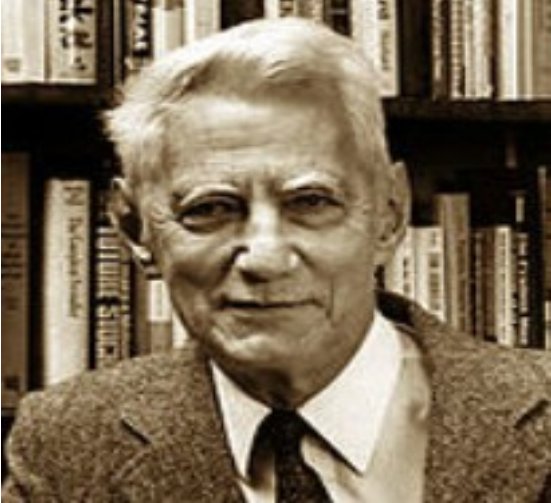
\includegraphics[width=2.8cm]{shannon.png}
	\begin{center}
		\vskip -0.3cm
		Клод Шеннон\\
		(1916--2001)
	\end{center}
\end{wrapfigure}
\noindent Мера Хартли подходит лишь для систем с равновероятными состояниями.
Если состояния системы S не равновероятны, используют меру Шеннона:
$$i(S)=-\sum_{i=1}^Np_i\cdot log_2p_i,$$
где N – число состояний системы,\\
\noindent рi – вероятность того, что система S находится в\\
состоянии i (сумма всех $p_i$ равна 1).
\vspace{0.2cm}
\begin{center}
	\color[rgb]{0,0.7,0.4}
	\textbf{Формула Хартли является частным случаем формулы Шеннона!}
	\color{black}
\end{center}
\noindent\textbf{Пример 1.} Количество информации в акте подбрасывания обычной монеты по формуле Хартли равно $\log_22=1$ бит. По формуле Шеннона получим то же $i_{s1}=-0,5*\log_20,5-0,5*\log_20,5=1$ бит.\\
\noindent\textbf{Пример 2.} При подбрасывании монеты со смещённым центром тяжести количество непредсказуемости становится меньше: $i_{s2}=-0,75*\log_20,75-0,25*\log_20,25\approx0,8$ бит.
\end{frame}